\begin{figure*}[ht]
  \centering

  \begin{subfigure}[b]{0.3\textwidth}
    \centering
    \begin{tikzpicture}[xscale=0.8]
      \drawclients{2}{5.5};
      \operation{1}{0}{2}{$w(0)$}{OK};
      \operation{2}{1}{3}{$w(1)$}{OK};
      \operation{1}{4}{5}{$r()$}{$0$};
    \end{tikzpicture}
    \caption{An example execution}\figlabel{LinearizableExampleNoLin}
  \end{subfigure}\hspace{12pt}
  \begin{subfigure}[b]{0.3\textwidth}
    \centering
    \begin{tikzpicture}[xscale=0.8]
      \drawclients{2}{5.5};
      \operation{1}{0}{2}{$w(0)$}{OK};
      \operation{2}{1}{3}{$w(1)$}{OK};
      \operation{1}{4}{5}{$r()$}{$0$};
      \notlinpoint{1}{1}{p0};
      \notlinpoint{2}{2}{p1};
      \notlinpoint{1}{4.5}{p2};
      \draw[notlinline, -latex] (p0) to (p1);
      \draw[notlinline, -latex] (p1) to (p2);
    \end{tikzpicture}
    \caption{An incorrect linearization}\figlabel{LinearizableExampleBadLin}
  \end{subfigure}\hspace{12pt}
  \begin{subfigure}[b]{0.3\textwidth}
    \centering
    \begin{tikzpicture}[xscale=0.8]
      \drawclients{2}{5.5};
      \operation{1}{0}{2}{$w(0)$}{OK};
      \operation{2}{1}{3}{$w(1)$}{OK};
      \operation{1}{4}{5}{$r()$}{$0$};
      \linpoint{2}{1.25}{p0};
      \linpoint{1}{1.75}{p1};
      \linpoint{1}{4.5}{p2};
      \draw[linline, -latex] (p0) to (p1);
      \draw[linline, -latex, bend right] (p1) to (p2);
    \end{tikzpicture}
    \caption{A linearization}\figlabel{LinearizableExampleGoodLin}
  \end{subfigure}

  \caption{}\figlabel{LinearizableExample}
\end{figure*}
